\chapter{Introduction} \label{chapitre-1}

Les concepts sur lesquels porte le travail décrit dans ce manuscrit sont définis dans cette première partie introductive. Tout d'abord, la technique du \glsfirst{nfb}-\glsfirst{eegi}, 
qui est au centre de ce travail, est présentée en détail, puis ses diverses applications sont listées. Dans la suite du manuscrit, seule l'une d'entre elles est étudiée : 
il s'agit du \glsfirst{tdah} chez l'enfant, dont les principales caractéristiques sont exposées dans cette partie. 

Une fois ces concepts décrits, les objectifs de cette thèse sont énoncés et la contribution de chaque chapitre est mise en évidence. Enfin, les analyses 
présentées dans ce manuscrit ont fait l'objet de publications scientifiques et d'une communication orale dont les références sont fournies à la fin de ce chapitre. 

\newpage 

\section{Définition du Neurofeedback}

Le \gls{nfb} est une technique d’apprentissage à visée thérapeutique permettant de modifier un paramètre d’activité cérébrale au moyen d’une 
information en temps réel, c'est à dire rendue instantanément, associée à un retour visuel ou auditif \citep{Arns2014} qui peut être délivré
dans le cadre d'un jeu sérieux \citep{Wang2010}. Une définition plus précise est donnée en \ref{principe_nfb}.

L'activité cérébrale peut être obtenue grâce à différents modes d'acquisition (\gls{fmri}, \gls{nirs}, \gls{ecog}, ...) comme détaillé par la suite, 
cependant celui qui nous intéresse ici est l'\glsfirst{eegie}, dont les caractéristiques sont tout d'abord
rappelées. Ensuite, la découverte et l'évolution de la méthode du \gls{nfb}-\gls{eegi} sont retracées, puis son principe est décrit précisément.

\subsection{Acquisition de l'électroencéphalogramme} \label{eeg_definition}

L'\gls{eegie} est un examen électrophysiologique du cerveau, non invasif, permettant d’enregistrer de manière amplifiée l'activité électrique du cerveau \citep{Nunez2006}. 

\subsubsection{Génération des signaux \gls{eegi}}

Cette activité cérébrale est enregistrée grâce à des électrodes placées sur le scalp qui détectent la sommation de l'activité électrique d'un grand nombre de neurones actifs de manière synchrone.
Cette activité électrique est générée par les potentiels post-synaptiques dans les dendrites apicaux des cellules pyramidales du cortex \citep{Hallez2007}. Le cortex désigne 
la substance grise périphérique des hémisphères cérébraux, il se compose de six couches qui comportent différents types de neurones : les cellules pyramidales à l'origine de l'\gls{eeg} 
se situent dans les couches III et V (la sixième étant la plus profonde). Ces cellules sont d'excellents dipôles électriques grâce à leur longue dendrite apicale perpendiculaire 
à la surface corticale \citep{Bekkers2011}. 

\subsubsection{Rythmes cérébraux}

L'\gls{eeg} est un signal de très faible amplitude (de l'ordre de 50$\mu$V) qui est d'ailleurs proportionnelle au degré de synchronisation des neurones pyramidaux \citep{Hallez2007}. 
Ainsi, en fonction de l'activité de ces neurones, différents rythmes cérébraux vont être présents sur l'\gls{eeg}. 

Les rythmes cérébraux correspondent à des oscillations électromagnétiques dans une bande de fréquences donnée, dont les bornes peuvent varier selon les études et sont présents sur l'\gls{eeg}
selon l'état psychologique d'un sujet \citep{Marzbani2016} :  
\begin{itemize}
\item \emph{les ondes delta} (moins de 4Hz) : observées lorsqu'un grand nombre de groupes de neurones est synchrone, c'est à dire pendant le sommeil profond,
\item \emph{les ondes thêta} (4-8Hz) : observées durant un état de somnolence, sous hypnose ou lors de la mémorisation d'informations par exemple,
\item \emph{les ondes alpha} (8-12Hz) : observées notamment durant un état de relaxation les yeux fermés,
\item \emph{les ondes bêta} (12-30Hz), dont les ondes \gls{smr} entre 12 et 15Hz : observées durant un état d'attention et de vigilance mentale par exemple,
\item \emph{les ondes gamma} (30-100Hz) : observées en particulier durant l'apprentissage.
\end{itemize}

Ces rythmes sont représentés à la Figure~\ref{Figure:introduction_EEG_waves}.

\begin{figure}[h!]
  \centering
	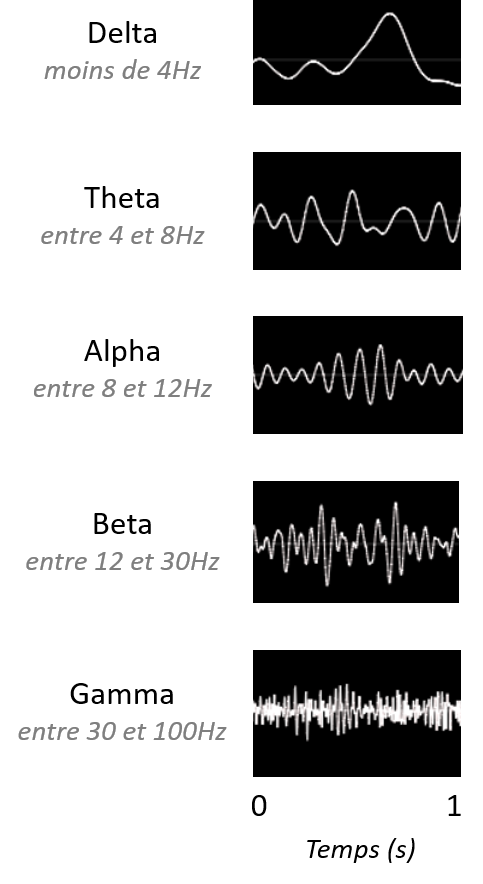
\includegraphics[width=0.5\linewidth]{figures/chapter-1/introduction-EEG-waves} 
  \caption[Rythmes cérébraux sur 1 seconde d'\gls{eeg} réel.]{Rythmes cérébraux sur 1 seconde d'\gls{eeg} réel. L'axe des ordonnées est entre -10 et 10$\mu$V.}
  \label{Figure:introduction_EEG_waves}
\end{figure}

\subsubsection{Aires cérébrales}

Afin d'interpréter la présence de ces rythmes cérébraux sur l'\gls{eeg}, il faut prendre en considération la zone sur laquelle ils sont observés 
car chaque aire cérébrale a des fonctions spécifiques, comme par exemple \citep{Marzbani2016} :
\begin{itemize}
\item \emph{la zone frontale} est impliquée dans la mémoire et la concentration,
\item \emph{la zone temporale} est impliquée dans le langage et la lecture,
\item \emph{la zone occipitale }est impliquée dans l'apprentissage visuel,
\item \emph{la zone pariétale} est impliquée dans la résolution de problèmes,
\item \emph{la zone centrale} est impliquée dans l'attention.
\end{itemize}

Ces différentes fonctions sont résumées à la Figure~\ref{Figure:introduction_cortical_areas_and_functions} où les principales électrodes, placées en accord avec le système \gls{eegi} 10-20 
défini par la suite, sont représentées ainsi que les aires cérébrales qu'elles couvrent. 

\begin{figure}[h!]
  \centering
	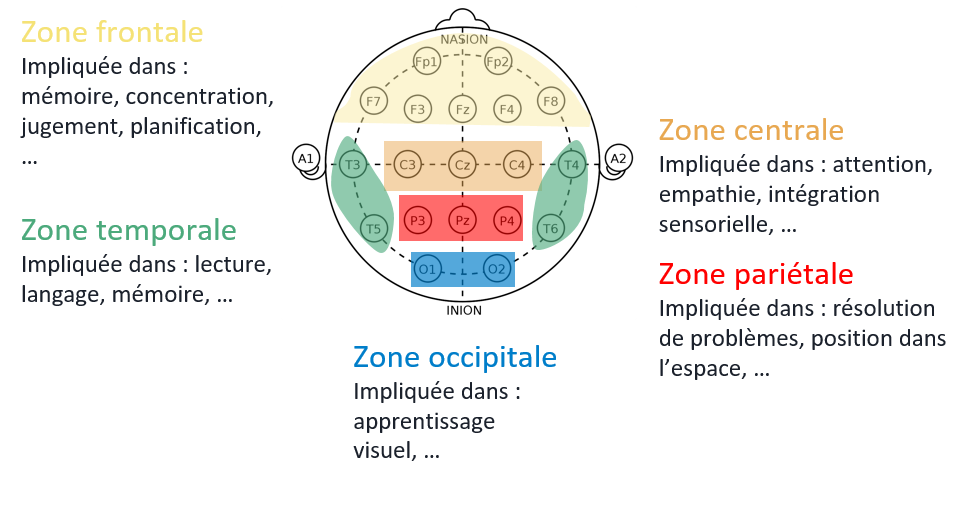
\includegraphics[width=1\linewidth]{figures/chapter-1/introduction-cortical-areas-and-functions} 
  \caption[Représentation des aires cérébrales avec des exemples de leurs fonctions.]{Représentation des aires cérébrales avec des exemples de leurs fonctions. 
	Les principales électrodes du système international 10-20 sont également présentées.}
  \label{Figure:introduction_cortical_areas_and_functions}
\end{figure}

\subsubsection{Enregistrement de l'\gls{eeg}}

L'\gls{eeg} est enregistré sur le cuir chevelu à l'aide d'électrodes dont le nombre et le placement varient en fonction de ce qu'on cherche à observer. L'\gls{eeg} correspond
au potentiel électrique entre deux points : l'électrode d'enregistrement et l'électrode de masse (\textit{ground electrode} en anglais). Cependant, cette dernière introduit
du bruit électrique, c'est pourquoi une électrode de référence est utilisée : le potentiel entre cette dernière et l'électrode de masse est mesuré puis soustrait à celui entre
l'électrode d'enregistrement et l'électrode de masse. Ainsi, l'\gls{eeg} reflète le potentiel entre l'électrode d'enregistrement et celle
de référence. L'emplacement de l'électrode de référence est variable : bout du nez, mastoïde ou une électrode d'enregistrement \citep{Michel2004}.

Le placement des électrodes suit généralement le système international 10-20 qui a été mis en place en 1948 afin d'harmoniser les enregistrements à travers le monde 
\citep{Jasper1949, Sharbrough1991} et qui est représenté à la Figure~\ref{Figure:introduction_system_10_20}.

\begin{figure}[h!]
  \centering
	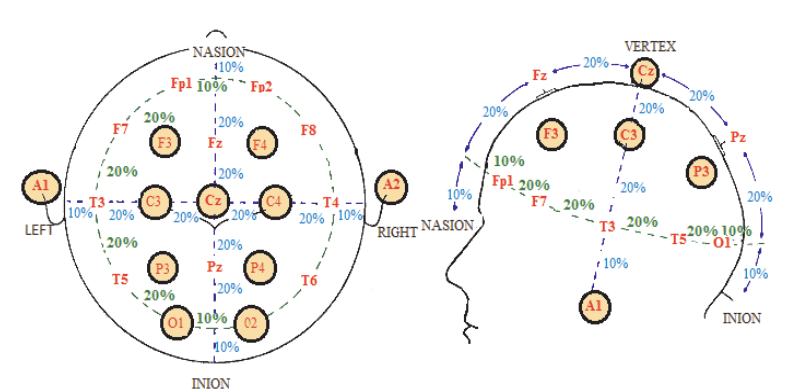
\includegraphics[width=1\linewidth]{figures/chapter-1/introduction-system-10-20} 
  \caption[Placement des électrodes enregistrant l'\gls{eeg} suivant le système international 10-20.]{Placement des électrodes enregistrant l'\gls{eeg} suivant le système international 10-20. 
	Les pourcentages sont calculés par rapport à la distance totale entre le nasion
	et l'inion, et par rapport à la distance totale entre les mastoïdes gauche et droit (A1 et A2). Les électrodes le plus couramment utilisées 
	sont cerclées de noir sur fond beige \citep{Marzbani2016}.}
  \label{Figure:introduction_system_10_20}
\end{figure}

Le système 10-20 couvre l'ensemble des aires cérébrales du cortex, en répartissant les électrodes de manière régulière entre les points de repère de la tête : le nasion (la 
dépression entre les yeux au sommet du nez), le vertex (le sommet de la tête) et l'inion (la bosse à l'arrière de la tête). 

Comme on peut le voir sur les Figures~\ref{Figure:introduction_system_10_20} et \ref{Figure:introduction_cortical_areas_and_functions}, le nom des électrodes est 
constitué d'une lettre et d'un chiffre ou de la lettre z, cette nomenclature est définie par \citet{Jasper1949} :
\begin{itemize}
\item la lettre renseigne la position de l'électrode sur le scalp : F, T, C, P et O correspondent respectivement aux régions Frontale, Temporale, Centrale, Pariétale et Occipitale,
\item le chiffre indique quant à lui si l'électrode est placée sur l'hémisphère droit (chiffre pair) ou sur l'hémisphère gauche (chiffre impair),
\item la lettre z est associée aux électrodes qui se trouvent sur la ligne médiane du crâne,
\item les électrodes Fp sont situées en pré-frontal,
\item les électrodes A1 et A2 sont généralement les électrodes de référence et de masse.
\end{itemize}
  
Le nombre et le placement des électrodes varient selon le but de l'application de l'\gls{eegie} : par exemple enregistrer l'\gls{eeg} afin
de mener une localisation de sources (c'est à dire déterminer les sources corticales à l'origine de l'\gls{eeg}) demande une forte densité spatiale \citep{Lantz2003}. 

Par ailleurs, le type des électrodes d'enregistrement peut également être différent : 
alors que les électrodes à gel sont considérées comme le \textit{gold standard}, l'utilisation des électrodes sèches se répand de plus 
en plus du fait notamment de leur facilité d'utilisation. Cependant, leur fiabilité n'est pas encore parfaitement démontrée \citep{Lopez2014}. 

Ce qui différencie les électrodes sèches des électrodes à gel est notamment la valeur de l'impédance qui, lorsqu'elle est faible, rend compte du bon contact entre la peau et les électrodes \citep{Lopez2014}. 
L'impédance est généralement obtenue en envoyant un faible courant de 10Hz entre 2 électrodes et en mesurant l'opposition à ce flux de courant \citep{Kappenman2010}. La peau du crâne est 
couverte par des cellules de peau morte qui conduisent à une forte impédance.
Ainsi, pour la diminuer, les électrodes à gel sont imprégnées d'un électrolyte qui facilite la transduction des courants ioniques. Toutefois, l'utilisation de ce type d'électrodes 
n'exclut pas la mesure de l'impédance qui doit être faible \citep{Lopez2014}. En général, en l'absence de gel conducteur, l'impédance se
situe entre 150 et 200 k$\Omega$ et tombe entre 5 et 10k$\Omega$ après application du gel \citep{Lopez2014}. Une faible impédance signifie 
que le niveau de bruit dans le signal est réduit \citep{Kappenman2010}.

Enfin, afin d'obtenir le tracé des signaux \gls{eegi} présenté à la Figure~\ref{Figure:introduction_eeg_example}, ceux-ci sont amplifiés 
à l'aide d'un amplificateur, qui peut être conforme à la norme ISO-60601-2-26 \citep{ISO}. Selon les systèmes d'acquisition utilisés, la fréquence
d'échantillonnage, qui correspond au nombre d'échantillons par seconde, est variable.

\begin{figure}[h!]
  \centering
	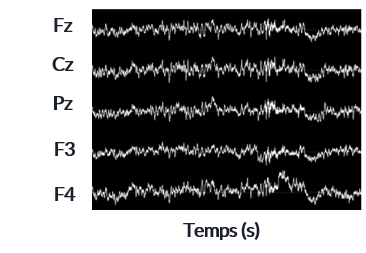
\includegraphics[width=1\linewidth]{figures/chapter-1/introduction-eeg-example} 
  \caption[Exemple d'\gls{eeg} réel enregistré sur 9 secondes.]{Exemple d'\gls{eeg} réel enregistré sur 9 secondes. L'axe des ordonnées est entre -40 et 40$\mu$V.}
  \label{Figure:introduction_eeg_example}
\end{figure}

\subsection{Exemples d'application de l'électroencéphalographie}

L'\gls{eegie} a diverses applications : il peut être analysé en différé, une fois que l'intégralité de l'enregistrement est disponible, notamment pour la localisation de sources \citep{Latif2006} 
mais aussi en temps réel dans le cadre, par exemple, de l'épilepsie, du suivi d'une personne dans 
le coma ou d'un enfant prématuré, du \gls{nfb}-\gls{eegi} et des interfaces cerveau machine (\gls{bci} en anglais) \citep{Li2010}. 

Les \gls{bci} et le \gls{nfb}-\gls{eegi} sont étroitement liés comme souligné par \citet{Jeunet2018} : dans les deux cas les utilisateurs doivent apprendre à réguler leur activité \gls{eegi} à l'aide du retour 
qui leur est délivré. Le but, pour un utilisateur de \gls{bci}, est de produire une activité cérébrale qui est traduite en une commande pour l'application de \gls{bci} lui permettant ainsi d'interagir 
avec son environnement \citep{Enriquez2017, Birbaumer2009}. Dans le cas du \gls{nfb}-\gls{eegi}, le but est d'apprendre à auto-réguler son activité cérébrale grâce au retour délivré en temps réel par l'application 
\citep{Enriquez2017, Jeunet2018} comme décrit en \ref{principe_nfb}.

Il existe différents types de \gls{bci} : les \gls{bci} dites actives, réactives et passives \citep{Mudgal2020}. Dans le premier cas, l'utilisateur essaye délibérément de contrôler son activité cérébrale afin
d'envoyer les commandes souhaitées à l'application, alors que dans le cas des \gls{bci} passives l'utilisateur n'a pas à contrôler son activité cérébrale, il doit seulement
se concentrer sur sa tâche : son activité est simplement analysée afin d'adapter le contenu de l'application de \gls{bci} \citep{George2014}. Quant aux \gls{bci} réactives, elles sont contrôlées 
par l'activité cérébrale obtenue en réponse à un stimulus extérieur.

Les applications des \gls{bci} actives sont diverses : les \gls{bci} peuvent être utilisées dans le cadre de jeux vidéo \citep{Kerous2018} mais aussi dans un but thérapeutique : remplacer ou
restaurer des fonctions utiles aux personnes handicapées suite, par exemple, à une blessure à la colonne vertébrale ou à un accident vasculaire cérébral \citep{Shih2012}. 

Les \gls{bci} réactives sont notamment utilisées pour aider les patients qui rencontrent des problèmes pour communiquer avec leur environnement \citep{Guy2018}. 

Quant aux \gls{bci} passives, elles peuvent être utilisées pour classifier des images grâce à l'activité \gls{eegi} ou pour évaluer la charge mentale \citep{George2014}.   

Dans le cadre de cette thèse, l'\gls{eeg} est enregistré et analysé en temps réel pour l'entrainement par \gls{nfb}-\gls{eegi} défini précisément par la suite.  
 

\subsection{Historique du Neurofeedback}

Les prémices du \gls{nfb}-\gls{eegi} remontent au début des années 1930, peu après l'enregistrement du premier \gls{eeg} humain et de la découverte des ondes alpha par Hans Berger en 1929 \citep{Berger1929}.
En effet, \citet{Durup1935} et \citet{Loomis1936} ont observé que les ondes alpha de l'\gls{eeg}, oscillant entre 8 et 12Hz, pouvaient être contrôlées grâce au 
conditionnement classique \citep{Pavlov1929}. Ce conditionnement, également appelé conditionnement répondant ou pavlovien, consiste à apprendre un comportement en associant un stimulus
de l'environnement à des réactions automatiques de l'organisme.

Plus tard, ce qui peut être considéré comme le premier entrainement par \gls{nfb}-\gls{eegi} a été mené par le Dr. Kamiya qui, en se basant sur les travaux de \citet{Durup1935}, 
a demandé aux sujets de son étude de contrôler le rythme alpha à l'aide d'un retour auditif \citep{Kamiya1969}, ce qu'ils ont réussi à faire. 

Une preuve solide de la modulation de l'\gls{eeg} a été rapportée dans les années 1960 par le Dr. Sterman et son équipe \citep{Sterman1969} : l'expérience 
originelle consistait à entrainer le cerveau des chats en leur apprenant quoi faire pour obtenir de 
la nourriture. En effet, les chats devaient dans un premier temps actionner un levier pour remplir leur bol de nourriture. Ensuite, une fois cette étape maitrisée, 
l'expérience s'est complexifiée avec l'ajout d'un son qui, lorsqu'il retentissait, empêchait les chats d'obtenir leur nourriture lorsqu'ils appuyaient sur le levier.
Une fois le silence revenu, le chat pouvait à nouveau recevoir de la nourriture en actionnant le levier.  

C'est durant cette phase de son expérience, au moment où le chat attend la fin du son, que le Dr. Sterman a extrait un rythme particulier au niveau de leur cortex sensorimoteur : 
le \gls{smr}, qui correspond aux fréquences entre 12 et 15Hz. Ensuite, le but du Dr. Sterman a été d'entrainer les chats à produire ce rythme en leur donnant de la nourriture, non plus grâce 
au levier, mais lorsqu'ils réussissaient à l'émettre pendant une demi seconde, ce que les chats ont vite appris à faire. Cette expérience a été la première à montrer que le comportement
du cerveau pouvait être affecté par la modulation de l'\gls{eeg}. 

Peu de temps après, le Dr. Sterman a été approché par la NASA pour évaluer la toxicité du carburant utilisé pour les fusées, connu pour son risque de provoquer de violentes crises
d'épilepsie, sur les astronautes. Afin de mettre en évidence son effet épileptogène, ce carburant a été testé sur des chats parmi lesquels ceux qui avaient précédemment appris 
à moduler leur \gls{smr}. Comme attendu, au contact de ce carburant, les chats
ont souffert de convulsions, mais ceux ayant participé à l'expérience du \gls{smr} ont présenté moins de crises ou ont eu une meilleure tolérance aux effets nocifs du carburant \citep{Sterman1974}.  
Cette expérience a permis de démontrer que le contrôle de l'activité cérébrale pouvait être associé à des bénéfices cliniques, ouvrant ainsi la voie aux expériences incluant les humains.

En 1972, une patiente épileptique a entrainé son \gls{smr} grâce à la technique du \gls{nfb}-\gls{eegi} : elle a réussi à moduler son \gls{smr}, conduisant à la quasi-disparition de ses crises 
d'épilepsie durant les séances \citep{Sterman1974}. 

Alors que l'épilepsie a été la première application du \gls{nfb}-\gls{eegi}, un autre usage thérapeutique possible commence à être étudié dans la foulée : l'hyperkinésie chez l'enfant \citep{Lubar1976ADHD}
qui peut être considérée comme l'ancêtre du \glsfirst{tdah} comme expliqué en \ref{adhd_history}. Cette étude est divisée en trois phases : tout d'abord, l'enfant module les ondes cérébrales d'intérêt 
dans le bon sens, puis ensuite dans le sens inverse et enfin à nouveau dans le bon sens. Des résultats encourageants sont observés.

A la suite de ces observations prometteuses, d'autres chercheurs se sont penchés sur cette technique, cependant, faute d'une technologie suffisamment puissante, il leur était impossible
d'obtenir des preuves cliniques plus solides. C'est pourquoi, après les années 80, le \gls{nfb}-\gls{eegi} est tombé en désuétude \citep{Masterpasqua2003}.
 
Il faut attendre les années 2000 pour que la communauté scientifique et médicale s'intéresse de nouveau sérieusement au \gls{nfb}-\gls{eegi}, conduisant à une explosion du nombre d'articles scientifiques publiés 
visant à mieux comprendre ses effets, illustrée à la Figure~\ref{Figure:introduction_number_of_nfb_publications}. 

\begin{figure}[h!]
  \centering
	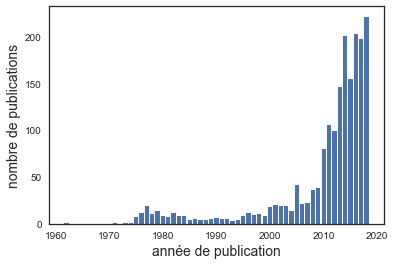
\includegraphics[width=0.7\linewidth]{figures/chapter-1/introduction-number-of-nfb-publications} 
  \caption[Evolution du nombre de publications sur le \glsfirst{nfb} par année, entre 1962 et 2018.]{Evolution du nombre de publications sur le \gls{nfb}-\gls{eegi} par année, entre 1962 et 2018. La base de données PubMed a été questionnée avec les 
	termes de recherche "Neurofeedback OR EEG Biofeedback".}
  \label{Figure:introduction_number_of_nfb_publications}
\end{figure}

Les dates clés de l'histoire du \gls{nfb}-\gls{eegi} sont résumées sur la frise présentée à la Figure~\ref{Figure:introduction_nfb_history}.

\begin{figure}[h!]
  \centering
	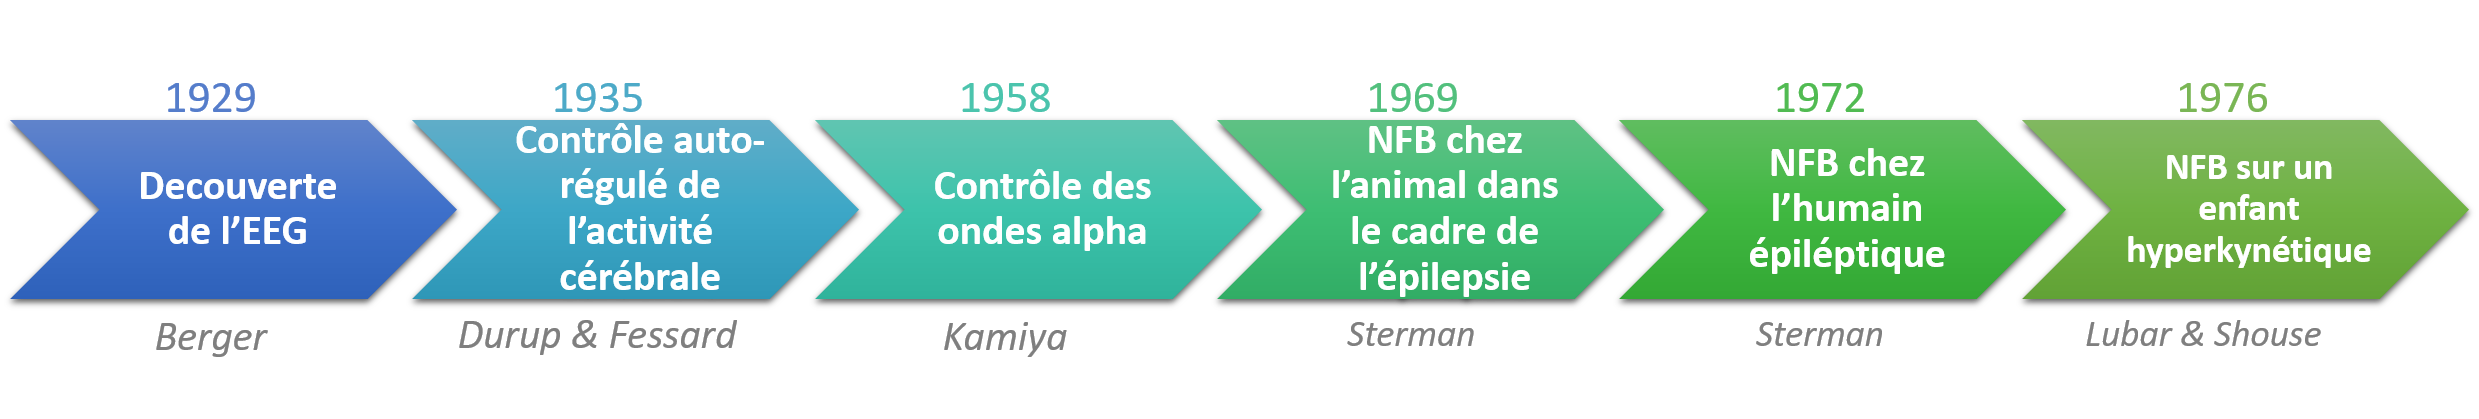
\includegraphics[width=1\linewidth]{figures/chapter-1/introduction-nfb-history} 
  \caption[Dates clés de l'histoire du \gls{nfb}.]{Dates clés de l'histoire du \gls{nfb}-\gls{eegi}.}
  \label{Figure:introduction_nfb_history}
\end{figure}

\subsection{Principe du Neurofeedback} \label{principe_nfb}

\subsubsection{Définition du \gls{nfb}}

Le \gls{nfb} a pour but d'apprendre à un sujet à auto-réguler son activité cérébrale à l'aide de retours auditifs, visuels et/ou tactiles en temps réel
intégrés dans un jeu sérieux \citep{Wang2010, Marzbani2016}. Ces retours lui permettent de suivre la régulation de son rythme cérébral instantanément : s'il est modulé de 
la manière souhaitée, une récompense auditive et/ou visuelle est attribuée, sinon le sujet doit prendre une action corrective. Une récompense visuelle
peut, par exemple, être la pêche d'un poisson \citep{Bioulac2019} et une récompense auditive un son agréable \citep{Strehl2006}

Le \gls{nfb} est basé sur le conditionnement opérant \citep{Reynolds1975} où le conditionnement n'est pas lié à 
des réponses réflexes de l'organisme, comme c'est le cas pour le conditionnement classique, mais à l'influence de l'environnement, qui 
renforce positivement ou négativement le conditionnement \citep{Skinner1948}. 

L'activité cérébrale enregistrée lors du \gls{nfb} est couramment l'\gls{eegie} dont les caractéristiques sont décrites en \ref{eeg_definition}.
Cependant d'autres modalités telles que, par exemple, 
l'\gls{ecog} \citep{Khanna2016, Gharabaghi2014}, la spectroscopie dans l'infrarouge proche (\glsfirst{nirs} en anglais) \citep{Marx2015} et 
l'Imagerie par Résonance Magnétique fonctionnelle (\gls{fmri} en anglais) \citep{Sulzer2013}
sont parfois utilisées. 

\paragraph{Electrocorticographie} 
L'\gls{ecog} enregistre l'activité cérébrale à l'aide d'électrodes implantées juste sous la boîte crânienne, en surface du cortex. Tout comme pour l'\gls{eegi}, 
les variations de potentiel électriques dues à l'activité neuronale sont mesurées \citep{Leuthardt2006}. 

\paragraph{\textit{Near-Infrared Spectroscopy}} 
Le \gls{nirs} mesure la corrélation entre l'hémodynamique et l'activité neuronale : la lumière dans l'infrarouge proche est absorbée de
façon différente selon la quantité d'hémoglobine oxygénée et désoxygénée ce qui permet de déterminer les changements de concentration relative
sur la surface corticale. Une forte activité cérébrale correspond à une concentration importante d'hémoglobine oxygénée \citep{Fallgatter1997, Marx2015}. 

\paragraph{\textit{functional Magnetic Resonance Imaging}} 
Le \gls{fmri} mesure la réponse \gls{bold}, c'est à dire les différences du signal dues à des changements locaux de la concentration d'hémoglobine désoxygénée 
dans le tissu cérébral qui est dépendante de l'activité neuronale \citep{Dewiputri2013}. Dans le cas du \gls{nfb}-\gls{fmri}, c'est à partir du signal 
\gls{bold} que le \textit{feedback} est calculé \citep{Dewiputri2013}. 

Alors que l'\gls{eegie} possède une résolution temporelle élevée, sa résolution spatiale est quant à elle faible, 
contrairement au \gls{fmri}. Ainsi des études ont implémenté un couplage de ces deux modalités pour pallier leurs faiblesses et conduire à des 
protocoles de \gls{nfb} plus efficaces \citep{Perronnet2017}. 

Cependant, bien que prometteur ce couplage est difficile à mettre en place, notamment à cause du \textit{feedback} \gls{fmri}.
Un couplage plus souvent observé est celui entre l'\gls{eegie} et l'\gls{emgie} : cette fois-ci le sujet doit réguler son activité cérébrale en même temps que son
activité musculaire et est donc récompensé sur les deux \citep{Bink2014}. \\
\\
\indent Le fait que l'\gls{eeg} soit la modalité le plus couramment utilisée pour l'entrainement par \gls{nfb} s'explique par sa bonne résolution temporelle, son caractère non-invasif
ainsi que par sa facilité de mise en place et son coût modéré \citep{Fovet2016}. Toutefois, comme évoqué plus haut, il souffre d'une mauvaise résolution 
spatiale et est sensible aux artefacts (mouvements physiologiques et bruits environnementaux) \citep{Iwasaki2005, Goncharova2003}. 

Dans la suite de ce manuscrit, seul le \gls{nfb}-\gls{eegi}, simplement noté \gls{nfb}, est étudié. 

\subsubsection{Etapes de l'entrainement par \gls{nfb}} \label{steps_NFB_taining}

Le \gls{nfb} est un entrainement cognitif en boucle fermée : une représentation de l'activité cérébrale est retournée en temps réel
au sujet afin de l'aider à la réguler \citep{Enriquez2017}. Cet entrainement s'effectue en cinq temps \citep{Enriquez2017}, détaillés
par la suite :
\begin{enumerate}
\item l'acquisition du signal \gls{eegi}, 
\item le pré-traitement en temps réel du signal,
\item l'extraction des marqueurs d'intérêt du signal qui doivent être modulés par le sujet (les neuromarqueurs),
\item la génération du \textit{feedback},
\item la modulation de l'activité cérébrale dont la stratégie est adaptée en fonction du retour reçu. 
\end{enumerate}

\paragraph{Acquisition du signal \gls{eegi}}
La première étape consiste à enregistrer l'\gls{eeg} comme expliqué précédemment dans la partie \ref{eeg_definition}. Le choix
du nombre et du placement des électrodes se fait en fonction de l'application du \gls{nfb}, dont les principales sont décrites en
\ref{applications_NFB}. 

Le signal \gls{eegi} étant de faible amplitude, il est très facilement perturbé par des artefacts d'origine physiologique (générés par le
corps du patient) et d'origine environnementale. Les artefacts physiologiques le plus couramment observés sont les clignements et mouvements
d'yeux \citep{Iwasaki2005} et les artefacts musculaires \citep{Goncharova2003} causés par exemple par des mouvements du visage ; les artefacts environnementaux sont le plus souvent 
dus aux lignes électriques (50Hz en Europe et 60Hz aux Etats-Unis). 

\paragraph{Pré-traitement en temps réel du signal \gls{eegi}}
Ces artefacts se superposent à l'activité électrique du cerveau pouvant fausser l'extraction du marqueur d'intérêt et donc rendre
incorrect le \textit{feedback} délivré \citep{Enriquez2017, Montgomery2001, Sherlin2011, Paluch2017}. C'est pourquoi des méthodes de rejet ou de correction d'artefacts en temps 
réel sont implémentées pour s'assurer que les récompenses sont bien calculées à partir du signal \gls{eegi} et non sur du bruit. 

Les méthodes de rejet consistent à ne pas extraire de marqueur d'intérêt d'un segment artefacté d'une durée donnée de l'\gls{eeg} (appelée époque). 
Pour sélectionner les époques à garder, certaines études définissent un seuil sur l'amplitude du signal : si l'amplitude du signal d'une époque est supérieure
à ce seuil, cette époque est rejetée \citep{Gevensleben2009, Heinrich2004}. La valeur de ce seuil peut être fixe ou adaptative et peut 
différer ou non selon les canaux. 

D'autres études se basent sur la géométrie Riemannienne pour rejeter les époques artefactés \citep{Barachant2013, Barthelemy2019, Bioulac2019}. 
La matrice de covariance de chaque segment, dont l'équation est donnée en équation Eq.~(\ref{eq:introduction_covariance_matrix}), est calculée pour un sous-ensemble de canaux (par exemple les canaux
centraux) : les segments dont la matrice de covariance se retrouve à l'extérieur d'une région d'acceptabilité définie grâce à une référence d'\gls{eeg} propres sont alors rejetés.

\begin{equation}
\label{eq:introduction_covariance_matrix}
\Sigma = \frac{1}{N - 1}XX^T,
\end{equation}
avec $X$ une matrice ($C \times N$) correspondant à une époque du signal \gls{eegi}, avec $N$ le nombre d'échantillons temporels et $C$ le nombre de canaux. 

Dans le cas où des artefacts sont détectés, l'utilisateur peut en être informé et adopter une action corrective, à l'instar de ce qui est implémenté dans 
\citet{Bioulac2019}.

Dans certains cas, les artefacts oculaires ne sont pas rejetés, mais sont corrigés en temps réel \citep{Barthelemy2017, Maurizio2014, Bioulac2019} en se basant sur
le principe de la séparation aveugle de sources (la \gls{bss} en anglais). Les signaux \gls{eegi} sont le résultat d'un mélange de sources cérébrales et non cérébrales : le but 
de la \gls{bss} est d'estimer ces sources à partir des signaux et d'identifier la source qui correspond à l'artefact oculaire pour la supprimer.
% équations ? plus de précisions ?

En ce qui concerne les artefacts électriques, ils sont corrigés à l'aide d'un filtre coupe-bande qui supprime le 50 ou 60Hz \citep{Bioulac2019}.

En résumé, trois approches sont envisageables pour traiter les artefacts :
\begin{itemize}
\item la détection/rejet des artefacts : seuil sur l'amplitude des signaux et géométrie Riemannienne,
\item la correction des artefacts : \gls{bss}, mais qui est difficile à implémenter en temps réel \citep{Barthelemy2017},
\item le couplage entre la correction et le rejet des artefacts : corriger les artefacts inévitables (les clignements d'yeux) 
et détecter/rejeter les artefacts évitables (les mouvements).
\end{itemize}

Traiter les artefacts est une étape essentielle du pré-traitement de l'\gls{eeg} : elle permet de délivrer à l'utilisateur un \textit{feedback} 
spécifique du marqueur \gls{eegi} à moduler lors de sa session de \gls{nfb} \citep{Barthelemy2019}. 

\paragraph{Extraction du marqueur d'intérêt}
Ensuite, la troisième étape consiste à extraire le marqueur à moduler lors de la session de \gls{nfb}, appelé par la suite neuromarqueur : 
celui-ci, tout comme les électrodes utilisées, dépend de l'application du \gls{nfb}. 

Le neuromarqueur correspond le plus souvent aux ondes cérébrales listées en \ref{eeg_definition}, isolées au 
niveau de certaines électrodes. Dans certains cas, le neuromarqueur est un ratio de deux ondes cérébrales \citep{Gevensleben2009}. C'est sur cette activité que le \textit{feedback}
est calculé. 

Les caractéristiques de l'\gls{eeg} étant différentes d'un sujet à l'autre, notamment à cause de l'âge, de la présence d'une maladie, de la capacité à effectuer une tâche ou du volume 
du cerveau \citep{Enriquez2017, Klimesch1999, Moretti2004, Alkoby2017}, la personnalisation des bandes de fréquences est parfois proposée par les applications de \gls{nfb}. 
En effet, il est supposé qu'adapter la définition des bandes de fréquences au sujet conduira à une meilleure efficacité \citep{Enriquez2017}. 

Une façon de personnaliser les bandes de fréquences est de se baser sur la fréquence du pic alpha du sujet 
\citep{Alkoby2017, Escolano2014, Bazanova2018, Bioulac2019}, appelée en anglais l'\gls{iapf}, qui 
est propre à chaque individu \citep{Haegens2014, Aurlien2004, Smit2006}. Un exemple de ce pic est présenté à la Figure~\ref{Figure:introduction_iapf}.

\begin{figure}[h!]
  \centering
	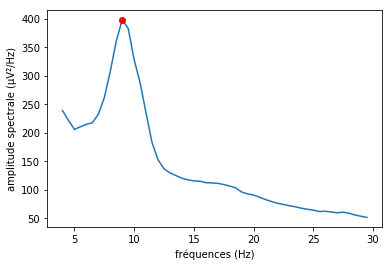
\includegraphics[width=0.7\linewidth]{figures/chapter-1/introduction-iapf} 
  \caption[Spectre d'un signal \gls{eegi} obtenu les yeux fermés au repos.]{Spectre d'un signal \gls{eegi} obtenu les yeux fermés au repos. L'\gls{iapf} correspond au point rouge.}
  \label{Figure:introduction_iapf}
\end{figure}

Enfin, certaines applications de \gls{nfb} proposent d'entrainer le neuromarqueur qui correspond le mieux au profil \gls{eegi} du sujet 
\citep{Bioulac2019, Kerson2013}, comme expliqué dans le cas du traitement du \gls{tdah} décrit en \ref{nfb_and_adhd}. 

\paragraph{Génération du \textit{feedback}}
Une fois le neuromarqueur extrait, l'étape suivante est de délivrer le \textit{feedback} au sujet. Pour ce faire, la valeur du neuromarqueur est comparée à un seuil
qui peut être fixe ou adaptatif, défini manuellement ou automatiquement \citep{Arns2014}.

En effet, le seuil peut être fixe tout au long de la session \citep{Kropotov2005, Monastra2002}, ou bien évoluer entre les sessions ou au sein même d'une session \citep{ 
Christiansen2014}. Utiliser un seuil incrémental a pour but d'adapter les récompenses octroyées au sujet en fonction de ses performances et 
de le garder motivé \citep{Bauer2016, Lansbergen2011}. La valeur du seuil peut être définie manuellement par un spécialiste ou bien automatiquement \citep{Arns2014}.

Le \textit{feedback} présenté au sujet dépend donc du résultat de la comparaison entre la valeur du neuromarqueur et celle du seuil. Par ailleurs, en fonction de la durée durant laquelle
le neuromarqueur est modulé comme souhaité, les récompenses peuvent varier \citep{Bioulac2019}. 

\paragraph{Modulation de l'activité cérébrale en fonction du \textit{feedback}}
Enfin, en fonction du \textit{feedback} qu'il reçoit, le sujet va moduler son activité cérébrale dans la direction attendue, en adaptant sa stratégie. 
Les caractéristiques des sujets qui réussissent à apprendre à contrôler correctement leur activité cérébrale, les \textit{learners}, ont fait l'objet de plusieurs études : 
\citet{Friedrich2014} note que ces derniers sont dans un état d'esprit positif et sont motivés. 

Le \textit{feedback} délivré peut-être visuel, auditif ou tactile ou bien combiné \citep{Vernon2004}.
\\
\\
Ces cinq étapes sont résumées à la Figure~\ref{Figure:introduction_nfb_explications}.

\begin{figure}[h!]
  \centering
	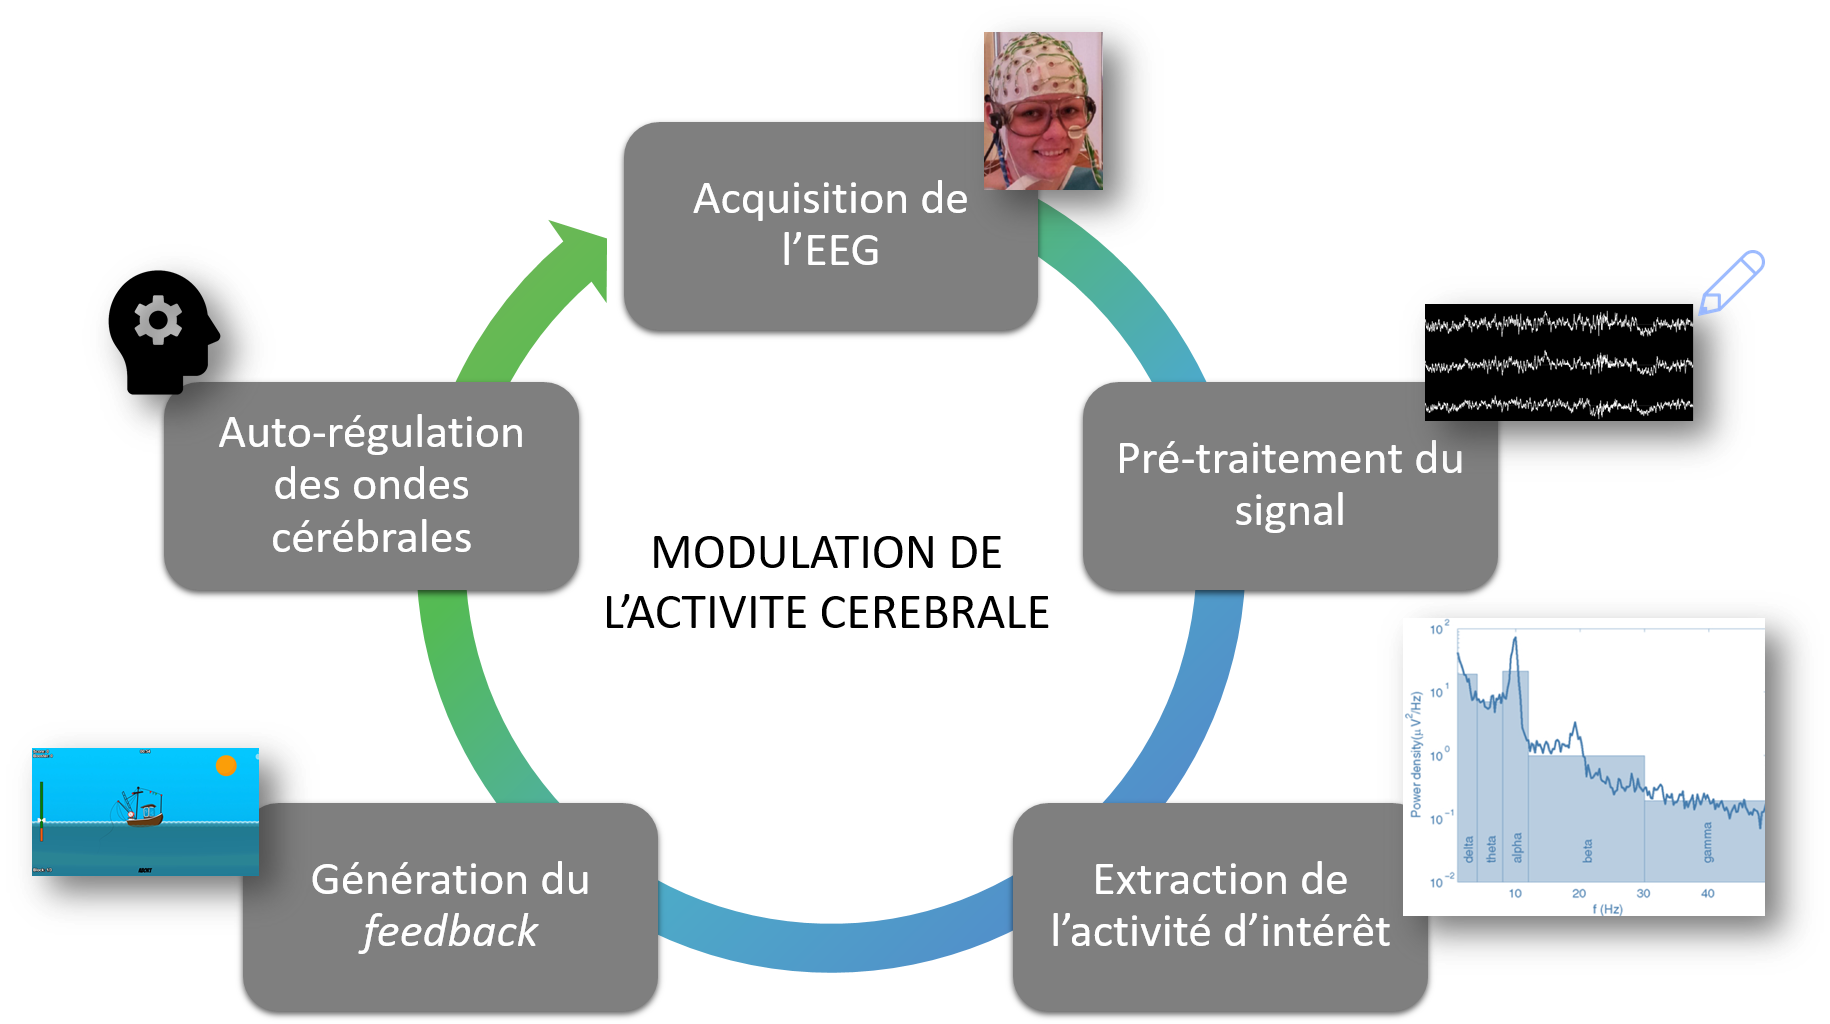
\includegraphics[width=1\linewidth]{figures/chapter-1/introduction-nfb-explication} 
  \caption[Schématisation du principe de \gls{nfb}.]{Schématisation du principe de \gls{nfb}.}
  \label{Figure:introduction_nfb_explications}
\end{figure}

\subsubsection{Déroulement du traitement par \gls{nfb}}

Une session de \gls{nfb} se divise généralement en plusieurs blocs d'entrainement de quelques minutes séparés par une courte période de repos.
Parmi ces blocs, certaines applications incluent 
un bloc dit de transfert durant lequel aucun retour n'est donné à l'utilisateur alors que celui-ci doit moduler son activité cérébrale \citep{Bioulac2019,
Bluschke2016, Gani2008, Strehl2006}. Cette phase de transfert a pour but de faciliter la transposition du contrôle appris durant les 
sessions de \gls{nfb} à la vie de tous les jours \citep{Arns2014}. Dans certains cas, afin d'aider cette transposition, une carte représentant l'interface du jeu sérieux est 
fournie au sujet afin qu'il puisse la regarder en modulant son activité cérébrale en dehors des sessions de \gls{nfb} \citep{Leins2007}.

L'entrainement par \gls{nfb} se compose de plusieurs sessions dont le nombre et la fréquence par semaine est variable, même lorsque le \gls{nfb} est appliqué au même trouble 
\citep{Enriquez2017}. La répétition de cet exercice de modulation cérébrale mène au phénomène de 
neuroplasticité \citep{VanDoren2017, Ros2010} qui est la capacité du cerveau de se modifier lors d'un apprentissage. Ce phénomène 
permet une réorganisation neuronale durable \citep{VanDoren2017}. 
%parler de la dopamine ? 

Un exemple de répartition des sessions sur une semaine d'entrainement ainsi qu'un exemple de déroulement d'une session de \gls{nfb} est représenté à la
Figure~\ref{Figure:introduction_timeline_session}. 

\begin{figure}[h!]
  \centering
	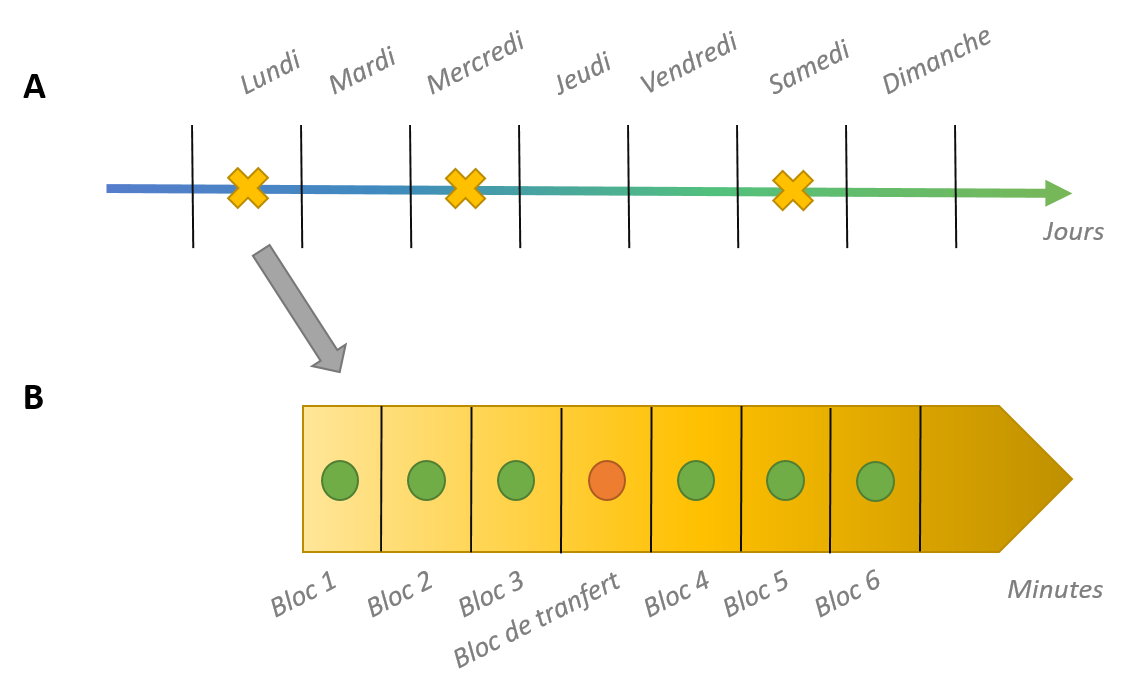
\includegraphics[width=1\linewidth]{figures/chapter-1/introduction-timeline-session} 
  \caption[Exemple de déroulement d'un traitement par \gls{nfb}.]{Exemples de répartition 
	des séances sur une semaine lors d'un entrainement par \gls{nfb} (en \textbf{A}) et du déroulement d'une session (en \textbf{B}). 
	En \textbf{A} Les croix jaunes correspondent aux jours où une session de \gls{nfb} est effectuée. En \textbf{B} les points verts représentent les blocs d'entrainement où un \textit{feedback}
	est délivré à l'utilisateur et le point orange au bloc de transfert où l'utilisateur n'a aucun \textit{feedback}.}
  \label{Figure:introduction_timeline_session}
\end{figure}

\section{Les champs d'application du Neurofeedback} \label{applications_NFB}

Le \gls{nfb} peut être utilisé dans différents cas dont les principaux sont détaillés ici \citep{Marzbani2016}. Parmi ces applications, l'une d'entre elles est présentée 
plus précisément car elle est exclusivement étudiée dans la suite de ce manuscrit : le \gls{tdah} chez l'enfant.

\subsection{De nombreuses applications} \label{NFB_applications}

Comme détaillé précédemment, l'\gls{eeg} comporte plusieurs composantes fréquentielles dont chacune correspond à une fonction physiologique différente.
En effet, par exemple, les ondes delta sont observées lorsque le sujet est endormi, les ondes thêta lorsqu'il somnole, les ondes alpha lorsqu'il est relaxé, 
les ondes bêta lorsqu'il est attentif et les ondes gamma lorsqu'il est en plein processus cognitif \citep{Marzbani2016}. 

Par ailleurs, la zone sur laquelle elles sont observées est également à prendre en considération, étant donné leurs fonctions différentes résumées
à la Figure~\ref{Figure:introduction_cortical_areas_and_functions}.

Certains troubles se caractérisent par un surplus ou un défaut d'un rythme cérébral dans une zone donnée, comme décrit par la suite. 
Ainsi, établir un protocole de \gls{nfb} consiste à identifier ces rythmes à moduler et l'aire 
du cortex à entrainer, et à déterminer s'il faut diminuer ou augmenter la présence de ce neuromarqueur, en se basant sur la littérature 
existante \citep{Micoulaud2019}.

Les applications du \gls{nfb} peuvent donc être assez diverses, les principales sont décrites ici. 

\subsubsection{Trouble du spectre autistique}

Le trouble du spectre autistique est un trouble neurodeveloppemental qui impacte considérablement les interactions sociales et qui est toujours présent à 
l'âge adulte. Les \gls{eeg} des enfants autistes présentent des anomalies comparés à ceux des enfants sains, notamment \citep{Coben2010, Kouijzer2010} :
\begin{itemize}
\item une activité dans les hautes fréquences de bêta liée à l'anxiété,
\item une forte activité du ratio delta/thêta correspondant à un déficit d'attention.
\end{itemize}
Lors de la plupart des entrainements par \gls{nfb} pour traiter le trouble du spectre autistique, il est demandé aux enfants de diminuer à la fois leur ratio 
thêta/alpha et d'augmenter la production d'ondes bêta dans l'aire centrale \citep{Thompson2010} et en pariétal, frontal et temporal \citep{Othmer2007}. 

\subsubsection{Epilepsie}

La recherche concernant le \gls{nfb} appliqué à l'épilepsie remonte au début de l'utilisation du \gls{nfb} avec \citet{Sterman1974}. Le protocole le plus
couramment utilisé est l'augmentation du \gls{smr} dans les zones centrales qui mène à une réduction du taux de crises 
d'épilepsie graves \citep{Hughes2008, Walker2010, Tan2009, Sterman2010}.

\subsubsection{Gestion de la douleur}

Le \gls{nfb} a également été étudié dans la diminution de la douleur en visant directement le traitement de la perception de la douleur. Le \gls{nfb} a, par
exemple, été utilisé dans le cas de lombalgies chroniques en entrainant les ondes alpha de façon à ce qu'elles soient synchrones sur l'ensemble des aires 
cérébrales \citep{Mcknight2001, Thapa2018, Mayaud2019}.

\subsubsection{Troubles du sommeil}

Le \gls{nfb} peut aussi être employé dans le cas de l'insomnie, trouble qui touche de nombreuses personnes \citep{Marzbani2016}. Plusieurs études se sont penchées sur ce traitement
basé sur l'augmentation du rythme \gls{smr} \citep{Schabus2014, Schabus2017}, cependant afin de conclure clairement quant à l'efficacité du \gls{nfb} davantage 
d'études contrôlées et en double aveugle sont nécessaires \citep{Micoulaud2019sommeil}. 

\subsubsection{Autres applications}

D'autres applications existent comme la diminution de l'anxiété via un protocole de diminution des ondes alpha \citep{Budzynski2009}, le traitement de la dépression
grâce à l'augmentation des ondes alpha et thêta tout en diminuant les ondes bêta \citep{Hurt2014} et l'augmentation de la concentration par le contrôle des ondes
alpha \citep{Babiloni2008, Berka2010}. Par ailleurs, le \gls{nfb} a également été appliqué dans le cadre de la rééducation suite à un accident vasculaire cérébral \citep{Biasiucci2018,
Cervera2018}. 

\subsubsection{Efficacité du \gls{nfb}}
 
Le \gls{nfb} est donc utilisé dans de nombreux cas mais son efficacité fait encore débat. Dans le cas de l'épilepsie, la méta-analyse de \citet{Tan2009}
montre que le \gls{nfb} conduit à une réduction significative de la fréquence des crises, cependant davantage d'essais cliniques
rigoureusement menés sont nécessaires avant de pouvoir conclure. 

Il en va de même dans le cas des douleurs chroniques où les résultats semblent prometteurs \citep{Mayaud2019} mais le manque d'études randomisées et
contrôlées empêche de
trancher sur l'efficacité du \gls{nfb}.

Ainsi, un des problèmes majeurs des études évaluant l'efficacité du \gls{nfb} est l'absence d'un groupe contrôle adéquat et le fait que les évaluateurs et sujets
ne soient pas aveugles \citep{Thibault2017, Thibault2017climate, Jeunet2018} empêchant ainsi de conclure quant à la spécificité du traitement par \gls{nfb}.

L'application du \gls{nfb} qui fait l'objet du plus grand nombre de recherches est le \glsfirst{tdah} chez l'enfant. Dans la suite de ce manuscrit seule 
celle-ci sera développée : elle est décrite précisément dans la section suivante.

\subsection{Neurofeedback et \gls{tdah}} \label{nfb_and_adhd}

\subsubsection{Définition du \gls{tdah}}

Le \gls{tdah} (ou \glsfirst{adhd} en anglais) est un trouble psychiatrique chronique qui touche environ 5\% d'enfants en âge d'aller à l'école, 
ce qui représente 2.5 millions d'enfants en Europe \citep{DSM-5}. En France, ce nombre se situe entre 3.5 et 5.6\% pour les enfants âgés de 6 à 12 ans \citep{Lecendreux2011}. 
Au niveau mondial, environ 3 à 7\% des enfants d'âge scolaire sont concernés par ce trouble. La plus forte prévalence se retrouve aux Etats-Unis où, selon certaines
études, 12\% des enfants et adolescents
sont diagnostiqués \gls{tdah} \citep{Collins2016}.

Ce trouble se caractérise par l'existence de trois groupes de symptômes \citep{HAS} : 
\begin{itemize}
\item le déficit attentionnel : l'enfant est dans l'incapacité de mener une tâche jusqu'au bout, il est distrait, il refuse ou évite les tâches qui demandent
une attention soutenue,
\item l'hyperactivité motrice : l'enfant ne cesse de s'agiter, il ne peut pas rester assis quand les conditions l'exigent, il fait preuve de peu d'organisation,
\item l'impulsivité : l'enfant a du mal à patienter, il a besoin d'agir et a tendance à interrompre les activités d'autrui, notamment en leur coupant la parole.
\end{itemize}
Pour certains enfants, un seul type de symptômes peut être prédominant, alors que d'autres les présentent tous de façon équivalente \citep{DSM-5} : 
on parle ainsi de présentation exclusivement inattentive, hyperactive ou mixte. Par ailleurs, de récentes 
études ont montré que les différents symptômes évoluent tout au long de la vie du patient \citep{CFDCAP, Epstein2013}. En effet, les symptômes du \gls{tdah}
peuvent perdurer jusqu'à l'âge adulte \citep{Faraone2006} : la prévalence des adultes souffrant de \gls{tdah} augmente \citep{Chung2019, Weibel2019}, 
ce qui en fait une problématique en plein essor. Toutefois, dans la suite du manuscrit, seul le \gls{tdah} chez l'enfant est étudié. 

En plus des symptômes décrits plus haut, le \gls{tdah} impacte négativement le bien-être des enfants : ceux-ci ont, pour la plupart, une faible estime d'eux-mêmes 
\citep{Shaw2005} et de mauvais résultats scolaires \citep{Barry2002}. Par ailleurs, ce trouble s'accompagne souvent de comorbidités telles que, par exemple, 
des troubles de l'humeur du comportement et de l'apprentissage \citep{Monastra2005}. Ainsi, afin d'être pris en charge de façon adaptée, il est 
important de diagnostiquer le \gls{tdah} au plus tôt. 

Ce trouble est majoritairement dû à un déséquilibre de certains neurotransmetteurs du cerveau, notamment du circuit dopaminergique, 
dit circuit de la récompense \citep{Daley2010, Punja2016}.Toutefois, les causes du \gls{tdah} ne sont pas encore claires et font l'objet de discussions
dans les différentes communautés scientifiques \citep{Galera2014}. En effet, des facteurs génétiques et environnementaux entrent en jeu comme par exemple le tabagisme ou le déficit en
vitamine D durant la grossesse et l'exposition à des pesticides durant la première année de vie de l'enfant \citep{Galera2014, Sucksdorff2019}.

En ce qui concerne les facteurs génétiques, des études montrent que le \gls{tdah} est fortement transmissible d'une génération à l'autre \citep{Larsson2014} :
dans les familles où un enfant a été diagnostiqué \gls{tdah}, plus de 30\% de frères et soeurs le sont aussi \citep{Monastra2005}.

Structurellement, des études \gls{fmri} et \gls{mri} ont montré des différences significatives au niveau de la taille et de la symétrie de régions cérébrales impliquées
dans l'attention entre les patients \gls{tdah} et sains au même âge, notamment au niveau du lobe frontal \citep{Monastra2005}.  

Enfin concernant le phénotype \gls{eegi} des enfants \gls{tdah}, \citet{Lubar1991} conclut que les enfants souffrant du \gls{tdah} présentent un excès 
d'ondes thêta en frontocentral \citep{Loo2010} et un déficit d'ondes bêta par rapport aux enfants sains du même âge ce qui a été confirmé par \citet{Barry2003}. Toutefois cette observation 
a été nuancée par \citet{Arns2012} qui précisent que seuls certains enfants \gls{tdah} présenteraient ce phénotype. 

\subsubsection{Histoire du \gls{tdah}} \label{adhd_history}

La première description des troubles de l'attention connue date de 1798. Il s'agit de celle de Sir Alexander Crichton qui donne dans son ouvrage 
une définition d'un trouble 
qui ressemble beaucoup au \gls{tdah} \citep{Crichton1798}, mais sans mentionner de symptômes d'hyperactivité : il s'intéresse seulement à l'attention
en la définissant par ailleurs de manière précise. 

En 1844, le Dr. Heinrich Hoffmann a écrit une série de petits livres pour enfants qui racontent l'histoire d'enfants dont l'agitation incessante 
entraine des conflits familiaux \citep{Lange2010}. Certains auteurs considèrent que ces livres contiennent la première description du comportement d'enfants 
souffrant du \gls{tdah} \citep{Burd1988, Kopf2006}.  

Pour beaucoup, le point de départ scientifique de l'histoire du \gls{tdah} sont les conférences tenues par Goulstonian de Sir George Frederic Still 
en 1902 \citep{Barkley2006, Conners2000, Palmer2001, Rafalovich2001} : il y expose le cas de 20 enfants présentant un défaut de contrôle moral sans
déficience intellectuelle ou maladie organique \citep{Still1902}. 

En 1932, les Dr. Franz Kramer et Hans Pollnow font état d'une "maladie hyperkinétique de l'enfance" dont le symptôme principal consiste en une 
activité motrice infatigable \citep{Kramer1932}. Ces symptômes avaient déjà été mis en évidence par le passé mais n'avaient pas été différenciés 
des maladies présentant des caractéristiques similaires, comme les symptômes résiduels de l'épidémie d'encéphalites léthargiques \citep{Lange2010}. 
Ainsi, les Dr. Franz Kramer et Hans Pollnow ont créé le concept de maladie hyperkinétique qui ressemble beaucoup à la définition actuelle
du \gls{tdah} \citep{Lange2010}. Peu de temps après, les premiers traitements médicamenteux sont mis au point : la prise d'amphétamines 
\citep{Bradley1937} et de psychostimulants \citep{Morton2000}. 

En 1968, la définition de la réaction hyperkinétique de l'enfance entre dans le \gls{dsm}-II, donnant ainsi une place centrale aux symptômes liés 
à l'hyperactivité. Cependant au cours des années 70, les scientifiques ont commencé à se focaliser sur le déficit de l'attention chez les enfants
hyperkinétiques. En effet, les déficits d'attention soutenue sont des caractéristiques plus significatives que l'hyperactivité 
\citep{Barkley2006, Douglas1972}. Ainsi dans le \gls{dsm}-III, la réaction hyperkinétique de l'enfance est renommée en "Déficit de l'attention 
avec ou sans hyperactivité" (\textit{Attention Deficit Disorder (ADD) (with or without hyperactivity)} en anglais). C'est en 1987 qu'apparait
l'acronyme \glsfirst{tdah} \citep{Lange2010}. 

Les dates clés de l'histoire du \gls{tdah} sont résumées sur la frise présentée à la Figure~\ref{Figure:introduction_adhd_history}.

\begin{figure}[h!]
  \centering
	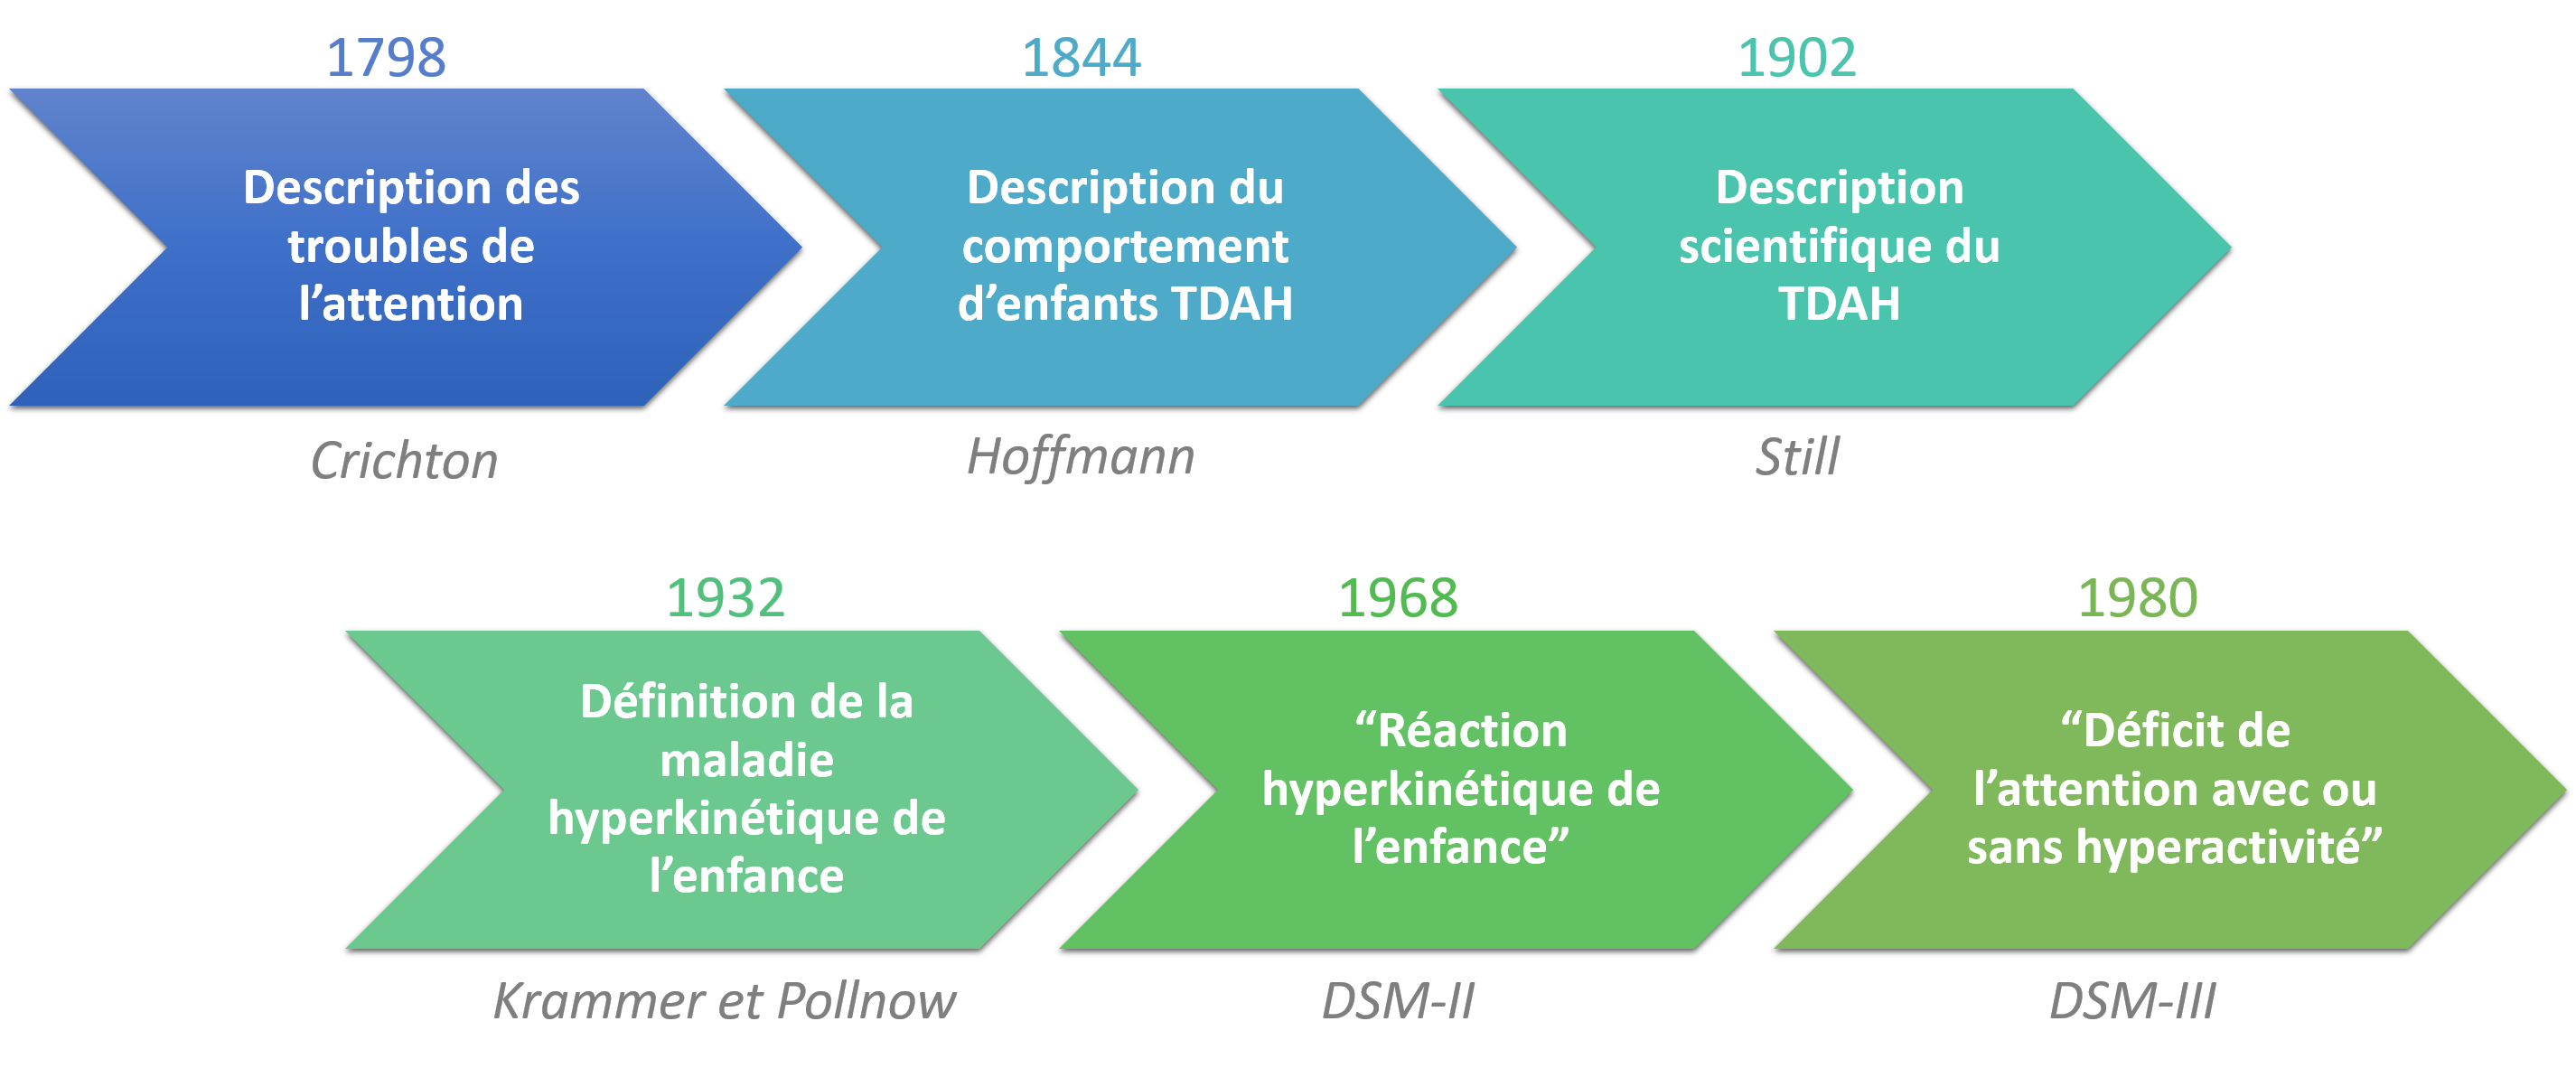
\includegraphics[width=1\linewidth]{figures/chapter-1/introduction-adhd-history} 
  \caption{Dates clés de l'histoire du \gls{tdah}.}
  \label{Figure:introduction_adhd_history}
\end{figure}

\subsubsection{Diagnostic du \gls{tdah}}

Le diagnostic du \gls{tdah} repose sur la clinique, des questionnaires évaluant le comportement de l'enfant peuvent être utilisés et être ensuite 
complétés par des mesures objectives de fonctions exécutives telles que les \textit{Continuous Performance Task} \citep{Barkley1991} à l'instar du 
\textit{Test of Variables of Attention} (TOVA) \citep{Forbes1998}.

En France, le diagnostic du \gls{tdah} est souvent établi par un spécialiste (neuropédiatre, pédopsychiatre ou neurologue en général).
Les critères cliniques sur lesquels se base le diagnostic du \gls{tdah} sont issus du \citet{DSM-5}.

Deux autres classifications caractérisent l'hyperkinésie de l'enfant, qui est un état d'hyperactivité, selon des critères et des postulats théoriques 
qui peuvent être différents : 
\begin{itemize}
\item la CIM-10 : Classification Internationale des Maladies proposée par l'Organisation Mondiale de la Santé,
\item la CFTMEA : Classification Française des Troubles Mentaux de l'Enfant et de l'Adolescent ayant un postulat psychodynamique.
\end{itemize}

L'apparition au cours de l'enfance et le caractère persistant des symptômes s'exprimant dans différents contextes de la vie de l'individu (en privé et 
en public) sont des critères fondamentaux pour le diagnostic du \gls{tdah} \citep{HAS}. Par ailleurs, les symptômes doivent porter préjudice au bon 
développement de l'enfant, aussi bien dans ses interactions sociales et familiales qu'au cours de son apprentissage. 

Un appareil ayant pour but d'aider le diagnostic du \gls{tdah} chez l'enfant en se basant sur leur \gls{eeg} 
a été approuvé par la \gls{fda} \citep{FDA, NebaHealth}, cependant les nouvelles études remettent en question l'utilisation de cet appareil \citep{Arns2013, 
Zhang2017}. Ainsi, des marqueurs objectifs cérébraux obtenus grâce à l'\gls{eegie} ou par \gls{fmri} ne permettraient pas d'améliorer le diagnostic pour un individu, mais
peuvent aider à distinguer différents groupes de patients \citep{Johnstone2005, Zhang2017, Clarke2011}. En effet, certains enfants \gls{tdah} 
présentent une augmentation d'ondes thêta et/ou une diminution d'ondes bêta dans l'aire frontale, ou une diminution du \gls{smr} dans l'aire centrale
\citep{Monastra2005, Janzen1995, Loo2018}. 

Le diagnostic du \gls{tdah} repose donc principalement sur des arguments cliniques basés sur les observations du comportement de l'enfant par le spécialiste 
mais aussi sur celles de ses parents et de ses enseignants, qui peuvent souffrir de
subjectivité et ainsi mener à des diagnostics erronés \citep{Lambez2019}.

\subsubsection{Traitements existants} \label{traitements_existants}

En France, la \citet{HAS} recommande en première intention une prise en charge non-médicamenteuse durant 3 mois à l'instar des thérapies cognitivo-comportementales. 
Ces thérapies se basent sur un système de récompenses pour encourager l'enfant à contrôler son \gls{tdah} \citep{Evans2011, Sonuga2004}.
Cependant, si ces approches se révèlent peu efficaces, un traitement médicamenteux peut être envisagé. En France seul le \gls{mph}
peut être prescrit en suivant des règles très strictes \citep{HAS}. Dans d'autres pays, d'autres molécules sont autorisées comme la lisdexamfetamine et 
les non-stimulantes tels que l'atomoxetine et la guanfacine \citep{Luan2017, Cortese2018}.

Même si le traitement médicamenteux est prescrit, la \citet{HAS} recommande de poursuivre les thérapies comportementales : un tel traitement multimodal 
est fortement conseillé dans le cadre du \gls{tdah} chez l'enfant.

Bien que très couramment utilisée,  la prise de \gls{mph} occasionne de fréquents effets secondaires,
notamment la diminution de l'appétit et des troubles du sommeil \citep{Sousa2012}. Ainsi, malgré son efficacité \citep{Taylor2014,
Storebo2015, Swanson2017, Cortese2018}, certains parents et médecins se tournent vers des alternatives non-pharmacologiques, comme par exemple les thérapies cognitivo-comportementales \citep{Berger2008} qui se révèlent néanmoins
moins efficaces que la prise de médicaments \citep{Sonuga-Barke2013}. 

Le \gls{nfb} est une autre approche non-médicamenteuse et non-invasive pour réduire les symptômes du \gls{tdah} \citep{Arns2015, Marzbani2016}.  
Plusieurs protocoles d'entrainement ont été proposés et étudiés :
\begin{itemize}
\item les protocoles basés sur les oscillations neuronales, qui visent à moduler la puissance dans des bandes de fréquences ciblées : augmentation du 
\gls{smr} généralement dans l'aire centrale \citep{Beauregard2006}, diminution du rythme thêta et/ou augmentation du rythme bêta dans les 
zones frontale et centrale \citep{Arns2015, Kropotov2005} ; lorsque ces deux dernières bandes sont contrôlées simultanément on parle du protocole 
\gls{tbr} \citep{Lubar1976, Arns2013}, 
\item les protocoles basés sur les \gls{scp}, qui consistent à réguler les seuils d'excitation corticale en se concentrant sur l'activité 
générée par des signaux extérieurs \citep{Heinrich2004, Banaschewski2007},
\item les protocoles basés sur les \gls{erp} : l'amplitude de l'onde P300 peut être considérée comme un marqueur neurophysiologique spécifique de l'attention 
sélective \citep{Desain2012, Fouillen2017, Arvaneh2019}. L'onde P300 est un \gls{erp} endogène, c'est à dire qu'il est lié à la réaction de la personne au stimulus et non aux 
caractéristiques de ce dernier. D'autres \gls{erp} peuvent être utilisés comme l'ont résumé \citet{Johnstone2013} et \citet{Barry2003erp}
\end{itemize}

Par ailleurs, les protocoles peuvent également être individualisés comme décrit en \ref{principe_nfb}.

\subsubsection{Efficacité du \gls{nfb} appliqué au \gls{tdah}}

La performance du \gls{nfb} dans le cadre du traitement du \gls{tdah} a fait l'objet de plusieurs études cliniques \citep{Escolano2014, Maurizio2014, Strehl2017} 
et de méta-analyses \citep{Arns2009, Arns2013, Sonuga-Barke2013, Micoulaud2014, Cortese2016, Catala2017, Lambez2019}. Dans ces études, l'efficacité du \gls{nfb} est 
principalement évaluée à l'aide d'échelles cliniques telles que, par exemple :
\begin{itemize}
\item ADHD Rating Scale \citep{Pappas2006},
\item Conners \citep{Conners2008},
\item SNAP-IV \citep{Bussing2008},
\item FBB-HKS \citep{Breuer2009},
\item BOSS Classroom Observation \citep{Shapiro2010}, 
\end{itemize}

Ces échelles se présentent sous la forme de questionnaires destinés aux parents, enseignants et médecins évaluant le comportement de l'enfant. 

Avant le début de l'entrainement par \gls{nfb}, les évaluateurs remplissent ces questionnaires dans le but d'obtenir un score rendant compte de 
la sévérité des symptômes : généralement, plus le score est haut, plus ils sont prononcés \citep{Pappas2006, Conners2008}. Par ailleurs, certaines échelles 
permettent de calculer un score pour les composantes inattention, hyperactivité et pour les symptômes totaux conduisant ainsi à une caractérisation 
plus précise du trouble \citep{Pappas2006}. Ces questionnaires sont ensuite remplis à l'issue de l'entrainement par les mêmes personnes afin de quantifier l'évolution 
des symptômes. 

Les évaluations des enseignants et des parents sont le plus souvent utilisées : bien que subjectives, elles sont tout de même considérées comme fiables 
\citep{Mcgough2004, Arns2020}. Les récentes méta-analyses décrivent les parents comme non-aveugles au traitement suivi par leur enfant (ils sont dits \gls{mprox}), alors
que les enseignants sont considérés comme probablement aveugles (\gls{pblind}) et donc potentiellement insensibles à un éventuel effet placebo 
\citep{Micoulaud2014, Cortese2016}. Cependant, des études ont montré qu'enseignants et parents n'évaluent pas de la même façon les symptômes du \gls{tdah}
\citep{Sollie2013, Narad2015, Minder2018, Enriquez2019, Arns2020}. En particulier les enseignants seraient plus sensibles à une amélioration
rapide des symptômes résultant généralement d'un traitement pharmacologique qu'à une diminution davantage étalée dans le temps, 
ce qui questionne sur la pertinence de se baser sur les évaluations \gls{pblind} pour mettre en évidence un 
effet placebo. De plus, \citet{Staff2020} observent, en corrélant les évaluations des symptômes par les enseignants à celles des pédiatres, que les premiers 
détecteraient plus aisément les symptômes liés à hyperactivité que ceux liés à l'inattention. Toutefois, les auteurs suggèrent que ce résultat 
pourrait également s'expliquer par le fait que les enseignants seraient sensibles à des symptômes d'inattention qui passeraient inaperçus lors 
des consultations médicales. 

Alors que les parents notent une amélioration significative des symptômes après l'entrainement par \gls{nfb} \citep{Arns2020}, les enseignants n'observent pas des
résultats aussi favorables \citep{Sonuga-Barke2013, Cortese2016}, ce qui ne permet pas de conclure clairement quant à l'efficacité du \gls{nfb}.
Par ailleurs, la plupart des études sur l'efficacité du \gls{nfb} appliqué aux enfants \gls{tdah} souffrent d'un faible nombre de patients inclus 
\citep{Baumeister2016, Heinrich2004} et de la difficulté, tant d'un point de vue technique qu'éthique \citep{LaVaque2001, Birbaumer1991, Holtmann2014} de mettre en place 
un groupe contrôle qui permettrait de démontrer la présence d'un éventuel effet placebo.

En effet, dans les études d'efficacité, le \gls{nfb} peut être comparé à différents types de contrôles \citep{Arns2014} :
\begin{itemize}
\item des contrôles aux conditions semi-actives qui visent à analyser les effets non-spécifiques du \gls{nfb} tels que l'importance de l'interaction entre le sujet et le thérapeute ; 
ces contrôles ne sont pas censés avoir un effet clinique sur le \gls{tdah}. Parmi ces contrôles, on trouve les thérapies cognitives ou le Biofeedback-\gls{emgic} qui renvoie un \textit{feedback} basé
sur l'activité d'un muscle donné \citep{Bakhshayesh2011},
\item des contrôles aux conditions actives qui, eux, sont connus pour avoir un effet clinique sur les symptômes du \gls{tdah} à l'instar d'un autre protocole de \gls{nfb} \citep{Leins2007} ou
de la prise de psychostimulants \citep{Meisel2014},
\item des contrôles aux conditions placebo, le \textit{sham}-\gls{nfb}, qui sont souvent considérés comme la référence absolue en recherche. Il s'agit d'un groupe contrôle
où tout est identique, sauf le \textit{feedback} qui n'est pas calculé sur l'activité électrique du cerveau \citep{Arnold2014}. Ce type de contrôle permet 
au sujet et à tous les évaluateurs d'être aveugles au traitement et donc de probablement éviter un effet placebo. Toutefois, un \textit{sham}-\gls{nfb} modifie 
la sensation de contrôle et donc l'éventuel effet placebo \citep{Kober2018}. 
\end{itemize}

Afin de confronter la performance du \gls{nfb} appliqué au \gls{tdah} aux autres traitements décrits en \ref{traitements_existants}, des histogrammes
représentant la distribution de l'efficacité de chaque traitement (quantifiée par une taille d'effet définie en \ref{es_within}) obtenue dans des études cliniques
sont tracés à la Figure~\ref{Figure:introduction-efficacy-treatments}.

Les études incluses pour le \gls{nfb} correspondent à celles sélectionnées suivant les critères d'inclusion présentés en \ref{selection_studies}, celles pour les
trois autres traitements (médicaments psychostimulants, médicaments non psychostimulants et thérapies comportementales) proviennent des plus récentes méta-analyses 
référencées sur PubMed sur le sujet au moment où ce travail a été effectué (été 2018) \citep{Luan2017, Catala2017}.

\begin{figure}[h!]
  \centering
	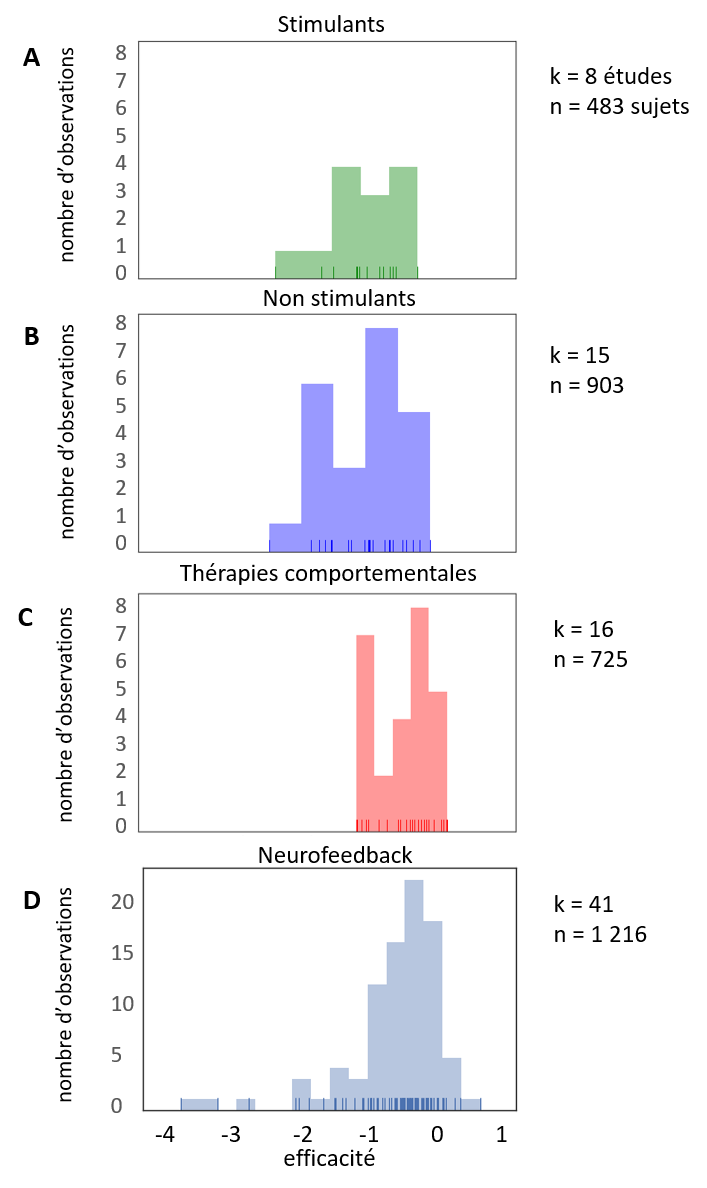
\includegraphics[width=0.5\linewidth]{figures/chapter-1/introduction-efficacy-treatments} 
  \caption[Visualisation de l'efficacité des traitement couramment utilisés dans le cadre du \gls{tdah}.]{Distribution de l'efficacité (définie ici comme la taille d'effet) 
	des traitements couramment utilisés pour les enfants \gls{tdah} à travers les études cliniques menées : 
	psychostimulants (\textbf{A}), non psychostimulants (\textbf{B}), thérapies comportementales (\textbf{C}), \gls{nfb} (\textbf{D}). k correspond au nombre
	d'études incluses et n au nombre de sujets. Une valeur d'efficacité négative est en faveur du traitement.}
  \label{Figure:introduction-efficacy-treatments}
\end{figure}

En analysant qualitativement ces histogrammes, on observe que les traitements médicamenteux (\textbf{A} et \textbf{B}) sont les plus performants, le \gls{nfb} (\textbf{D}) présente de bons
résultats, en partie meilleurs que les thérapies comportementales (\textbf{C}). 

L'efficacité du \gls{nfb} sur le long terme a fait l'objet de quelques études, mais avec un nombre de sujets qui reste plutôt faible. Il est observé notamment
que l'entrainement par \gls{nfb} des enfants \gls{tdah} conduit à une amélioration de la mémoire de travail encore présente un an après la fin du traitement
\citep{Dobrakowski2019}. Par ailleurs, la diminution des symptômes du \gls{tdah} chez les enfants ayant effectué du \gls{nfb} reste stable 6 mois après 
l'intervention contrairement aux enfants ayant pris du méthylphénidate \citep{Gelade2018}. Une méta-analyse incluant dix essais contrôlés randomisés comparant l'efficacité du \gls{nfb}
à celle des traitements semi-actifs et actifs montre que, six mois après la fin du traitement, les effets du \gls{nfb} sont supérieurs à ceux du groupe contrôle semi-actif
et équivalents à ceux du traitement actif \citep{VanDoren2019}.  

La spécificité du traitement par \gls{nfb} fait également débat \citep{Ros2019, Schonenberg2017} : comme décrit précédemment, en se basant sur les évaluations des parents, 
la plupart des études rapportent une diminution des symptômes du \gls{tdah} chez les enfants ayant effectué un entrainement par \gls{nfb}. Or, 
une façon de déterminer si ces changements de comportement résultent
effectivement de ce traitement serait de mettre en évidence une différence entre la valeur du neuromarqueur (souvent sa puissance spectrale) à pré et à post-test ou avec
le groupe contrôle à post-test. 
\citet{Gevensleben2009eegeffects} et \citet{Janssen2016randomized} se sont penchés sur l'évolution de la valeur du neuromarqueur et concluent tous deux 
à la spécificité du \gls{nfb}. Cependant, cette conclusion est nuancée
par les résultats d'une étude s'intéressant à l'évolution de la puissance spectrale du neuromarqueur six mois après la fin du traitement par \gls{nfb} \citep{Janssen2020} : les auteurs
n'observent aucune différence entre la puissance spectrale du neuromarqueur extrait chez les enfants ayant effectué du \gls{nfb} et celle des enfants ayant pris du 
\gls{mph}.  

Enfin, comme tout traitement, le \gls{nfb} peut provoquer des effets secondaires notamment de la fatigue, des maux de tête, de l'anxiété, des perturbations du sommeil et de l'irritabilité qui
sont généralement observés dans les 24 à 48h suivant la séance et se dissipent au-delà \citep{Hammond2007}. 


\section{Objectifs de la thèse}

Le \gls{nfb} a fait l'objet de nombreuses études pour déterminer son efficacité dans le cadre du \gls{tdah} chez l'enfant comme souligné précédemment.
Malheureusement, aucun consensus n'a encore été clairement atteint, ainsi le travail effectué au cours de cette thèse a pour but de déterminer les facteurs 
de réussite de l'entraînement par \gls{nfb} pour les enfants \gls{tdah} en se basant sur des données cliniques mais aussi physiologiques. 

Les trois sous-objectifs de ce travail, chacun développé dans un chapitre, sont les suivants :
\begin{itemize}
\item étudier l'efficacité du \gls{nfb} chez les enfants souffrant du \gls{tdah} à l'aide d'une méthode couramment utilisée : la méta-analyse,
\item identifier les paramètres méthodologiques, techniques et cliniques influençant la performance de ce traitement,
\item analyser la distribution d'un marqueur de l'attention (le \gls{tbr}) au sein d'une population d'enfants \gls{tdah} pour mieux cibler
l'entrainement par \gls{nfb}. 
\end{itemize}

\section{Contribution et résumé des chapitres}

Ce manuscrit est divisé en cinq parties, dont les trois centrales (les chapitres \ref{chapitre-2}, \ref{ch-saob} et \ref{chapitre-4}) 
ont chacune pour but de remplir un des objectifs précédemment énoncés.

Avant de chercher à déterminer les facteurs de réussite de l'entrainement par \gls{nfb}, son efficacité sur les enfants \gls{tdah} est évaluée à l'aide 
d'une méthode couramment utilisée \citep{Sonuga-Barke2013, Micoulaud2014, Cortese2016} et présentée dans le chapitre \ref{chapitre-2} : la méta-analyse. 
Les résultats de ce type d'analyse ont un impact important sur la communauté scientifique : \citet{Micoulaud2016} a notamment réagi à la méta-analyse de 
\citet{Cortese2016} en discutant certains points de cette analyse. 

Ainsi, dans ce chapitre la méta-analyse de \citet{Cortese2016} qui, au moment où ce travail a été mené était la plus récente sur le sujet, 
est répliquée en modifiant les points qui ont fait débat \citep{Micoulaud2016} afin de jauger leur impact sur les conclusions émises dans la méta-analyse. 
Ensuite, étant donné que de nouvelles études satisfaisant les critères d'inclusion établis par \citet{Cortese2016} sont disponibles, cette méta-analyse 
est mise à jour : en plus des 13 études originellement incluses, 7 sont ajoutées, ce qui apporte une plus grande puissance statistique aux résultats. 
La réplication et la mise à jour sont effectuées, non pas avec les logiciels 
habituellement utilisés tels que RevMan \citep{Revman}, mais à l'aide d'un package Python développé pour cette occasion et disponible en ligne afin de favoriser 
la réplication et/ou la mise à jour de ce travail \citep{Bussalb2019c}. 

La réplication de la méta-analyse conduisant aux mêmes résultats que \citet{Cortese2016}, les choix discutés par \citet{Micoulaud2016} n'ont pas un impact assez
important pour changer ses conclusions : le \gls{nfb} est jugé efficace par les parents alors que les enseignants, considérés comme \gls{pblind}, ne notent aucune
amélioration significative. Par ailleurs, la mise à jour confirme les résultats de \citet{Cortese2016}, ce qui laisserait penser qu'ils commenceraient
à se figer. En outre, l'évolution de l'\glsfirst{est} (défini en \ref{compute_summary_effect}) et de sa $p$-value en fonction de l'ajout des nouvelles études selon
leur année de publication est tracée afin de mettre en évidence une éventuelle stabilisation des résultats. 

Ce chapitre a été l'occasion de mener une revue de littérature des études d'efficacité sur le \gls{nfb} appliqué aux enfants \gls{tdah} 
qui a permis de mettre en évidence la forte hétérogénéité d'un point de vue clinique et méthodologique de ces études. 

Alors que la fiabilité des résultats des méta-analyses souffre de ces différences qui pourraient, par ailleurs, expliquer l'absence de consensus quant 
à l'efficacité du \gls{nfb} \citep{Alkoby2017}, une analyse en tirant avantage est implémentée ici : la \gls{saob} décrite dans le chapitre \ref{ch-saob}. 

Les facteurs méthodologiques et/ou cliniques fortement variables entre les études tels que, par exemple, la durée du traitement, le nombre de sessions et le type 
de protocole de \gls{nfb} suivi, sont extraits de 41 études d'efficacité sur le \gls{nfb} appliqué aux enfants \gls{tdah}, dans le but de déterminer lesquels 
ont un impact sur l'efficacité du \gls{nfb}. Pour ce faire, trois méthodes de régression multivariées sont utilisées : la \glsfirst{wls}, le \glsfirst{lasso} et le \gls{dt}. 

La \gls{saob} identifie trois facteurs qui semblent avoir un impact sur l'efficacité du \gls{nfb} : 
\begin{itemize}
\item un traitement intensif semblerait préférable, 
\item l'intégration d'une phase de transfert aurait un impact négatif, 
\item les évaluations des enseignants seraient plus
sévères quant à l'amélioration du traitement. 
\end{itemize}

Le package Python développé pour mener la \gls{saob} est disponible en ligne afin de permettre facilement la réplication et la mise à jour 
de ce travail \citep{Bussalb2019c}. 

La personnalisation des protocoles de \gls{nfb} est un facteur innovant dont il aurait été intéressant d'étudier l'impact sur l'efficacité du \gls{nfb}.  
Cependant, faute d'un nombre suffisant d'études ayant recours à la personnalisation, ce facteur n'a pas pu être étudié dans la \gls{saob}. C'est pourquoi
la pertinence d'une personnalisation est étudiée dans le chapitre \ref{chapitre-4} grâce à l'analyse de la distribution d'un marqueur de l'attention : 
le \gls{tbr} pour lequel de précédentes études ont montré qu'il serait variable au sein de la population d'enfants souffrant de \gls{tdah} \citep{Zhang2017, Arns2013, Clarke2001}.

Les valeurs de \gls{tbr} sont extraites de 363 \gls{eeg} d'enfants \gls{tdah} et vont être partitionnés grâce à trois méthodes : le \glsfirst{bgmm}, le partitionnement
hiérarchique basé sur la distance de Ward et le \glsfirst{dbscan}. Si la distribution est trouvée bimodale par ces trois méthodes, les seuils calculés par chaque méthode,
sont comparés, notamment grâce à une courbe \glsfirst{roc} obtenue sur
les résultats du \gls{bgmm} à deux composantes afin de déterminer celui qu'il faudrait utiliser pour attribuer le protocole de \gls{nfb}.

Les trois méthodes s'accordent sur le fait que la distribution des \gls{tbr} est bimodale, ce qui indique qu'il existe en effet deux groupes d'enfants
\gls{tdah} : l'un présentant des \gls{tbr} plutôt faibles et l'autre avec des \gls{tbr} élevés. Ainsi, personnaliser le protocole de \gls{nfb} en 
fonction de la valeur de \gls{tbr} semblerait pertinent, mais son efficacité n'a pas été étudiée ici. Après comparaison des seuils \gls{tbr} obtenus, 
celui de 4.1 apporterait le plus d'équilibre entre 
un faible taux de faux positifs et un taux de vrais positifs élevé. Cette analyse a également souligné l'existence de nombreuses
façons de calculer le \gls{tbr}, ainsi elle a permis d'établir une recommandation sur la définition du \gls{tbr} à partir de laquelle nos
résultats ont été obtenus. 

\section{Liste des publications}

Le travail décrit dans ce manuscrit a donné lieu aux publications avec comité de lecture suivantes :

\begin{description}
\item \citet{Bussalb2019tbr} : A. Bussalb, S. Collin, Q. Barthélemy, D. Ojeda, S. Bioulac, H. Blasco-Fontecilla,
D. Brandeis, D. P. Ouakil, T. Ros, and L. Mayaud. Is there a cluster of high
theta-beta ratio patients in attention deficit hyperactivity disorder ? \textit{Clinical Neurophysiology}, 2019a.
\item \citet{Bussalb2019clinical} : A. Bussalb, M. Congedo, Q. Barthélemy, D. Ojeda, E. Acquaviva, R. Delorme,
and L. Mayaud. Clinical and experimental factors influencing the efficacy of
neurofeedback in ADHD: a meta-analysis. \textit{Frontiers in psychiatry}, 10 :35, 2019b.
\end{description}

Les résultats de \citet{Bussalb2019clinical} ont été mis à jour dans ce manuscrit.

Une partie des travaux de \citet{Bussalb2019clinical} ont fait l'objet d'une communication orale :
\begin{description}
\item A. Bussalb, M. Congedo, R. Delorme, E. Acquaviva, Q. Barthelemy, D. Ojeda, J.A. Micoulaud-Franchi, L. Mayaud. Neurofeedback 
appliqué aux enfants TDAH : quels facteurs influencent son efficacité ? 6ème Congrès de la SOFTAL, mai 2018. 
\end{description}
